\documentclass[letterpaper,twocolumn,openany,nodeprecatedcode]{dndbook}

% Use babel or polyglossia to automatically redefine macros for terms
% Armor Class, Level, etc...
% Default output is in English; captions are located in lib/dndstrings.sty.
% If no captions exist for a language, English will be used.
%1. To load a language with babel:
%	\usepackage[<lang>]{babel}
%2. To load a language with polyglossia:
%	\usepackage{polyglossia}
%	\setdefaultlanguage{<lang>}
\usepackage[english]{babel}
%\usepackage[italian]{babel}
% For further options (multilanguage documents, hypenations, language environments...)
% please refer to babel/polyglossia's documentation.

\usepackage[utf8]{inputenc}
\usepackage[singlelinecheck=false]{caption}
\usepackage{lipsum}
\usepackage{listings}
\usepackage{shortvrb}
\usepackage{stfloats}
\usepackage{tikz}
\usetikzlibrary{mindmap,trees,shadows,decorations.pathmorphing}

\captionsetup[table]{labelformat=empty,font={sf,sc,bf,},skip=0pt}

\MakeShortVerb{|}

\lstset{%
  basicstyle=\ttfamily,
  language=[LaTeX]{TeX},
  breaklines=true,
}

\title{The Final Exam \\
\large at school for enterprising henchmen }
\author{Adam Saleh}
\date{2020/04/21}

\begin{document}

\mainmatter%

\section{The Final Exam at the school for enterprising henchmen}

\DndDropCapLine{A}{s your final task} you are to guard \emph{the MacGuffin} situated on an altar in a cave where you will be teleported in a short while.
There is an annual festival in a small town an hour south from the cave, where heroes and adventurers from the county gather to try their luck with delving into the cave.
As long as \emph{the MacGuffin} is still on the altar y sunrise, your class have passed the exam. On behalf of the entire faculty, I wish you luck. Your evaluation begins now!
\emph{a portal opens and the headmaster waves you through}

\subsection{How to play this?}

This is a one-shot adventure for the simple \emph{Dice v. Dice} system.
It should be easy to use this with many other systems, that deal well with improvisational tone,
like Fate or Powered by the Apocalypse, and bit trickier for ones that live on statted encounters, like D\&D.


\subsubsection{The Dice v. Dice System}

{To play, have}
\begin{itemize}
  \item an idea of your world
  \item players, each with idea of a character
  \item 2 distinct 20-sided dice
\end{itemize}

You describe \emph{the world}. They describe \emph{their characters} actions.

Anytime consequence is uncertain, agree on one possible outcome for each die. Roll. Higher die wins.

\subsubsection{Idea for the world}

The world for this adventure is a one of twisted but whimsical fairy-tale.
Think of Alice in Wonderland, the world of Shrek movies or The Adams Family.
A world where bad-guys have an evil university and adventurers go dungeon-delving for sport.

\subsubsection{Choosing Characters}

Because the system is very free-form, players character should have a singular strong concept to help guide them,
for example:
\subparagraph{The Witch} And old angry grandmother, in black robe with a pointy hat. Can transform others into objects and animals on a whim.

\subparagraph{The Zombie} Hard to kill, but easy to dismember walking corpse. Requires supply of brain-matter to keep functioning, absorbing the personality of the previous owner of said brain. Has small stash of brains.

\subparagraph{The Ogre Thief} Raised by gnomes to be a thief, thinks he is just an oversized gnome. Intimidates people to maintain the illusion of stealth. Has a large box to put the loot in.


\subsection{The situation}

Your players' characters are just before the final exam in the school for enterprising henchman, hoping to pass,
so they get the certificate needed to be hired by local evil over-lords.

\subsubsection{Characters know ...}
they need to guard \emph{the MacGuffin} in the cave until the sun-rise.

\subparagraph{The Cave}
Has large empty space and small altar with \emph{the MacGuffin} in the middle. There are boxes with disguise kits, if there was a need to venture incognito into the village for some reason.

\subparagraph{The Dropout}
Last to walk through the portal is a student they haven't seen before. Supposedly they are repeating the exam from the last year.

\subparagraph{The Town Festival}

There is a festival in the village, celebrating the heroes and adventurers about to delve into the cave to get \emph{the MacGuffin}.

\subsubsection{... in reality}
there are several misdirects.

\subparagraph{The Town Festival} If the adventurers succeed to get \emph{the MacGuffin} they return back to \emph{the Festival} to celebrate, giving your students of evil one last chance to take it back. What they don't know unless they venture to \emph{the Festival} that it is a carnival, where everybody except for the adventurers are dressed up as their favorite monsters.

\subparagraph{The Situation} The town is fake. The festival is organized by the school and the heroic adventurers are in fact alumini helping out the head-master with the exam. There is a magic barrier around the entire area to prevent outside interference.

\subparagraph{The Dropout is Faculty} Either the headmaster or some other faculty joined the students in disguise to aid in their evaluation. They should subtly help the adventurers get \emph{the MacGuffin}, forcing the students to venture out of the cave to save it.

\subsection{Areas}

\centering
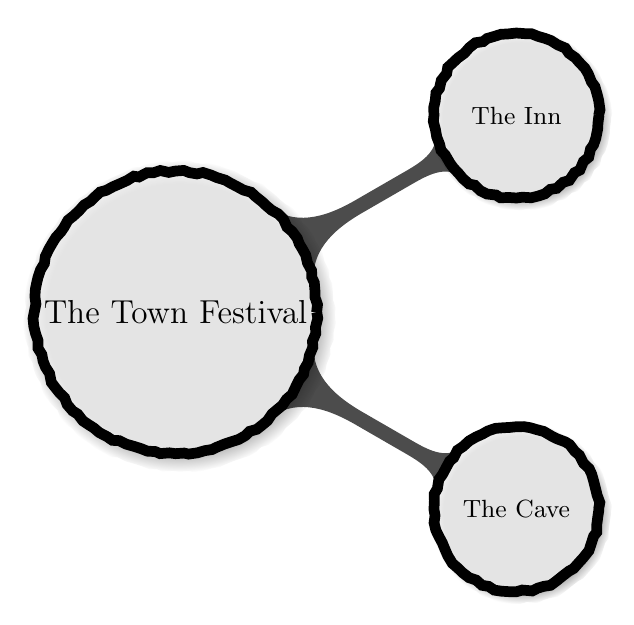
\begin{tikzpicture}
  \begin{scope}[mindmap, grow cyclic,
every node/.style={concept, circular drop shadow, minimum size=0pt},
concept/.append style={
  concept color=black, fill=white, fill opacity=0.7, text opacity=1, line width=0.9ex, text=black,
decorate,
  decoration={random steps,segment length=0.6ex,amplitude=0.12ex}},
text=white
    ]
    \node[concept] {The Town Festival}
    child[concept] {
      node[concept] {The Cave}}
    child[concept] {
      node[concept] {The Inn}
    };
  \end{scope}
\end{tikzpicture}

The town is unreasonably short walk from the cave. Most of the town is engaging in festivities of The Festival.
There is a single small inn, with cheap beer on tap and half-decent meals, where adventurers gather before they embark.

\DndArea{The Cave}
%https://commons.wikimedia.org/wiki/File:Kozarnika_cave_-_entrance.jpg
\frame{\includegraphics[width=1.0\linewidth]{./img/cave.jpg}}
The cave has a big entrance that is hard to barricade and a single large cavern.

\DndArea{The Festival}
\frame{\includegraphics[width=1.0\linewidth]{./img/festival.jpg}}

The festival. Think more of a Fashung or Mardi Gras, than a halloween party.

\DndArea{The Inn}
% https://commons.wikimedia.org/wiki/File:Fren%C5%A1t%C3%A1t_pod_Radho%C5%A1t%C4%9Bm_(4).jpg
\frame{\includegraphics[width=0.9\linewidth]{./img/rathaus.jpg}}

% https://commons.wikimedia.org/wiki/File:Hospoda_interier_TMB.jpg
\frame{\includegraphics[width=0.9\linewidth]{./img/hospodas.jpg}}

If \emph{the students} venture into the town early, they would found adventurers in the local inn.

\end{document}
